\section{Frontend Structure}

\begin{figure}[H]
    \centering
    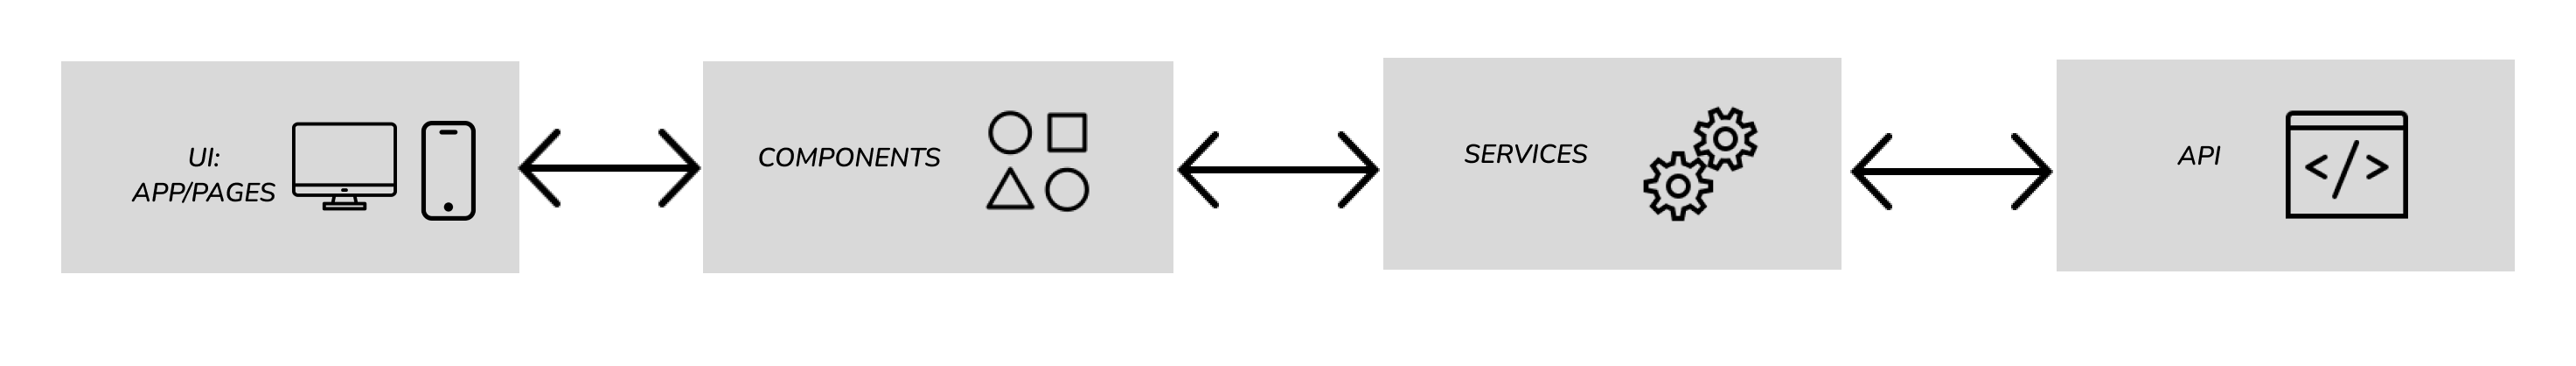
\includegraphics[width=1.05\textwidth]{img/frontend_structure.png}
    \caption{Frontend Structure}
    \label{fig:web-frontend-structure}
\end{figure}

The frontend structure is organized into three main directories:
\begin{itemize}
    \item \textbf{app:} This directory contains the main application logic, routing, and top-level components that orchestrate the application flow.
    \item \textbf{components:} This directory is dedicated to reusable UI elements and some specific components that are used in the application.
    \item \textbf{services:} This directory handles business logic, data fetching, interactions with the backend API, and other functionalities that need to be shared or separated from the UI components.
\end{itemize}


\section{Components}
The components are the main building blocks of the frontend. They are used to create the UI of the application, they are not associated with a specific page which means they are reusable.

They are organized in the \texttt{components} directory, when one is used in multiple pages it is placed in the \texttt{ui} directory, these ui components are mainly imported from shadcn/ui. The components are organized by the page they are used in, for example the \texttt{dashboard} directory contains components used in the dashboard page like the \texttt{walletOverview} and \texttt{expenseChartItem} components.


\subsection{State Management}
Our application relies on a structured state management approach to ensure data consistency and component reactivity. We implemented a hybrid strategy combining local component state with global application state management.

At the component level, we leverage React's useState hook for managing local state such as form inputs, loading states, and temporary UI interactions. For application-wide state that needs to be shared across multiple components, we implemented a context-based architecture using React's useContext hook.

The core of our global state management centers around the \texttt{WalletContext}, a custom context provider that maintains the user's wallet collection and tracks the currently selected wallet. This centralized approach ensures that wallet-related data remains synchronized across all components that depend on it. See more details on the context implementation in Section \ref{sec:contexts_web}.

We deliberately chose this combination over more complex state management solutions like Redux or state machines. While state machines offer powerful state transition control, our use case primarily involves managing straightforward data flows and form states. The useState approach provides sufficient flexibility for handling complex forms, such as the transaction creation form, where we manage both service-fetched data and user input validation simultaneously.

\subsection{Components Interaction}
The components are organized in a way that allows them to interact with each other. For example, the \texttt{limits} component uses the \texttt{limitsCarousel} component to display the limits of the different categories. In this case the \texttt{limits} component is the parent and the \texttt{limitsCarousel} component is the child, which means that all the data that the \texttt{limitsCarousel} component needs is passed as props in the \texttt{limits} component, sometimes callbacks are passed to the child component to handle the user interactions as shown in the example below.

\begin{lstlisting}[caption={Limits Component child component}, label={lst:limits-component-child}]
<LimitCarousel
    limits={limits}
    onEditClick={handleEditClick}
    onDeleteClick={handleDeleteClick}
/>
\end{lstlisting}

This way the father component has the ability to control the child appearance and behavior through props. When there are new information to be displayed in the child component, the father component can pass the new information as props and the child component will be able to use it to render the new information.

\subsection{API Interactions}
In order for the components to have the data they should display, they need to call the services that fetch the data from the API. This is done by using the useEffect hook, which is a hook that is used to fetch the data when the component is mounted or when a specific state of the component changes. The next example shows how the \texttt{limits} component fetches the data from the API.

\begin{lstlisting}[caption={Limits Component useEffect}, label={lst:limits-component-useEffect}]
useEffect(() => {
    setIsLoading(true);
    const fetchData = async () => {
        try {
            const [newLimits, categories] = await Promise.all([
                limitService.getLimits(walletId, limit, offset),
                CategoryService.getCategories(walletId)
            ]);
            setLimits(newLimits);
            setAllCategories(categories);
        } catch (error) {
            console.error("Error fetching data:", error);
        } finally {
            setIsLoading(false);
        }
    };
    fetchData();
}, []);
\end{lstlisting}

\section{Report}

To provide users with better control over their finances, we implemented a customizable report generation feature using PDF generation. Before addressing the technical implementation, we first decided between client-side and server-side approaches. We chose client-side generation for several reasons: it reduces server load, enables real-time user feedback during the generation process (displaying progress indicators like "fetching transactions", "processing categories", "generating charts"), and offers better scalability for an application with potentially many users generating reports concurrently.

With this decision made, we then faced the challenge of incorporating graphics into PDFs. After research and testing, we considered the two most common approaches:
\newpage
\begin{itemize}
    \item \textbf{Approach 1: Render graphics in the DOM and capture them as images for the PDF.} \\
    This method involves creating the visualizations using standard rendering techniques (e.g., charts via libraries like Recharts or Chart.js), taking a screenshot of them (e.g., with \texttt{html2canvas}), and embedding the resulting image in the PDF. We also found some personal projects from developers who faced the same problem and created libraries to automate this process. However, since these libraries could be discontinued or their usage might be restricted in the future, we decided not to consider them.

    \textbf{Pros:}
    \begin{itemize}
        \item Faster to implement, as it leverages existing visualization libraries.
        \item Minimal need to manually manage graphical layout or rendering logic.
    \end{itemize}
    
    \textbf{Cons:}
    \begin{itemize}
        \item Unreliable results: screenshots often failed or captured incomplete content.
        \item Lower quality and resolution, especially when scaling or printing.
        \item Limited styling control once the image is captured.
    \end{itemize}
    
    \item \textbf{Approach 2: Generate graphics directly in SVG and include them in the PDF.} \\
    This alternative involves writing logic to build and render the graphics directly as SVG elements, which are then embedded into the PDF.

    \textbf{Pros:}
    \begin{itemize}
        \item Full control over layout, styling, and rendering.
        \item High-quality output that scales well for printing.
        \item More reliable and consistent integration into the PDF.
    \end{itemize}
    
    \textbf{Cons:}
    \begin{itemize}
        \item Requires additional development effort to implement custom rendering logic.
        \item Increased complexity when we need advanced visuals(pie charts, bar charts, etc).
    \end{itemize}
\end{itemize}

After evaluating both approaches, we opted for the second one due to its superior flexibility, quality, and reliability—despite the extra development effort required to manually build the SVG graphics.




\section{Contexts} \label{sec:contexts_web}
In the React framework, contexts are used to share data between components without the need to pass props through the entire component tree. This is especially useful when the same data needs to be accessed across multiple views. In our implementation, we use several contexts, but the most important one is the \texttt{WalletContext}, which stores both the selected wallet and the list of all wallets belonging to the user. This is essential because most of our main components need access to this data.

We treat this context like a cache, allowing us to access wallet information without making repeated API calls. This is particularly helpful on the dashboard page, where wallet data needs to be available at all times.

To implement this properly, we created a \texttt{WalletProvider} component. It wraps the parts of the application that need access to the wallet context. This component handles the state for both the wallets and the selected wallet. It fetches data from the API, stores it in the context, and provides it to the components that depend on it. Here's what the return statement of the \texttt{WalletProvider} component looks like:

\begin{lstlisting}[caption={WalletProvider}, label={lst:wallet-provider}]
    return (
        <WalletContext.Provider
          value={{
            currentWallet: currentWallet!,
            wallets,
            loading,
            changeWallet,
            changeBalance,
            editWallet,
            deleteWallet,
            ...
          }}
        >
          {children}
        </WalletContext.Provider>
      );
\end{lstlisting}

As shown above, the \texttt{WalletProvider} component returns a \texttt{WalletContext.Provider}, which supplies the selected wallet, all wallets, and a set of functions to manage them. When the provider is mounted, it fetches the wallets from the API and stores them in the context.

To make it easier to use this context in components, we also created a custom hook called \texttt{useWallet}. This hook allows components to access wallet data without having to directly use \texttt{useContext(WalletContext)}. Here's an example of how it's used:

\begin{lstlisting}[caption={useWallet}, label={lst:use-wallet}]
const { currentWallet, wallets, loading, changeWallet, changeBalance, editWallet, deleteWallet } = useWallet();
\end{lstlisting}

The useWallet hook was created so the components that need to access the wallets or the selected wallet can do it without having to use the \texttt{useContext(WalletContext)}. Here is the implementation of the useWallet hook.

\begin{lstlisting}[caption={useWallet hook}, label={lst:use-wallet-hook}]
    export const useWallet = (): WalletContextType => {
        const ctx = useContext(WalletContext);
        if (!ctx) {
          throw new Error('useWallet must be used within WalletProvider');
        }
        return ctx;
      };
\end{lstlisting}

There are other contexts that are used in the application such as: 

\begin{itemize}
    \item \texttt{RegisterContext} that is used to store the email of the user when the user is registering.
    \item \texttt{ThemeContext} that is used to store the theme of the application.
\end{itemize}

\section{Middleware}
To help user experience and prevent unauthorized access to protected frontend pages, we implement a Next.js middleware\cite{nextjs-middleware} that handles authentication-based routing decisions. This middleware operates exclusively on frontend page routes, ensuring users are properly directed based on their authentication status without interfering with API endpoint functionality, this middleware only checks if the token exists in the cookies and if it does it redirects to the dashboard page and then the backend checks if the token is valid, since we can't have the value of the cookies via typescript, if the token does not exist it redirects to the home page.

\begin{lstlisting}[caption={Middleware}, label={lst:middleware_frontend_web}]
const publicRoutes = ['/', '/register', '/register/confirmEmail'];

export function middleware(request: NextRequest) {
    const { pathname } = request.nextUrl;
    const isPublicRoute = publicRoutes.some(route => pathname === route);
    const token = request.cookies.get('token')?.value;

    if (!isPublicRoute && !token) {
    return NextResponse.redirect(new URL('/', request.url));
    }

    if ((pathname === '/' || pathname === '/register') && token) {
    return NextResponse.redirect(new URL('/dashboard', request.url));
    }

    return NextResponse.next();
}

export const config = {
    matcher: ['/((?!api|_next|.*\\..*).*)'],
};
\end{lstlisting}

The middleware intercepts requests to frontend pages and evaluates the user's authentication status through cookie-stored tokens. It automatically redirects users to appropriate pages based on their authentication state, creating a seamless navigation experience while maintaining security boundaries for protected content.

\textbf{Important Note:} This middleware specifically excludes API routes (as defined by the matcher configuration). The middleware focuses solely on frontend page routing and user experience optimization.

\subsection{Architecture Components}
\textbf{Route Classification System:}
The publicRoutes array defines frontend pages accessible without authentication, including the home page (/), user registration (/register), and email confirmation (/register/confirmEmail) routes. This centralized configuration allows for easy modification of public access permissions as the application grows.

\textbf{Selective Route Matching:}
The matcher configuration ensures the middleware only processes frontend page requests while excluding:
\begin{itemize}
\item API routes (\texttt{/api/*})
\item Next.js internal routes (\texttt{/\_next/*})
\item Static assets (files with extensions like \texttt{.css}, \texttt{.js}, \texttt{.png}, etc.)
\end{itemize}
This selective approach prevents interference with API functionality and static resource serving.

\textbf{Token-Based Authentication Check:}
The middleware extracts authentication tokens from HTTP cookies to determine user authentication status. This approach provides a server-side validation mechanism that works seamlessly with Next.js's server-side rendering capabilities.

\textbf{Intelligent Page Redirection:}
The system implements smart redirection logic for optimal user experience:
\begin{itemize}
\item Unauthenticated Access Protection: Users without valid tokens attempting to access protected frontend pages are redirected to the home/login page, preventing access to sensitive areas like user dashboards or account pages.
\item Authentication Flow Optimization: Users with valid tokens who navigate to login or registration pages are automatically redirected to the dashboard, eliminating redundant authentication steps and improving user flow.
\end{itemize}

\textbf{Request Continuation:}
When no redirection conditions are met, the middleware allows requests to proceed normally using NextResponse.next(), maintaining standard Next.js routing behavior for all appropriate scenarios.

This middleware architecture focuses specifically on frontend user experience and page-level access control, while API security remains the responsibility of individual endpoint implementations.